\IEEEPARstart{N}{owadays} searches look at facial features detection, and facial expression recognition. Indeed, for analyse a face there is several methods. Principal Component Analysis (PCA), Linear Discriminant Analysis (LDA), and Locality Preserving Projection (LPP) are most used methods \cite{Using-Graph}.In this part, we will quickly present each typical methods employed for analyse a face\cite{Active-Shape}. These approchs are not used alone, they are often combinated.\\
	
	
	\subsection{Principal Component Analysis (PCA)} \leavevmode\par
	PCA is a useful statistical technique that has found application in fields such as face recognition and image compression, and is a common technique for finding patterns in data of high dimension. For use PCA, we need to have several images available. PCA represent images such as this :
		\begin{itemize}
		\item For an image I (nxn), there is $n^{2}$ pixels.
		\item For k images PCA extract $n^{2}$ k-dimensional vectors.	
		\item After that PCA reduce vector space dimension. The result of the five step of PCA give us a simple way to know if two images are neighbor.
		\end{itemize}
	
	Now we have an average image, wich is a concept. If we use a learning method, for create an average face with each basic images. With all of these average faces, we create a covariance matrix. Now we can calculate eigenfaces and we project base's visages in eigenfaces' subspace.
	And to finish compare Euclid distance of images.
		
		
	\subsection{Linear Discriminant Analysis (LDA)}
	The linear discriminant analysis (LDA) is used to find the linear combination of features that is the best separation between
object classes or events. The resulting combinations can be used
as a linear classifier, or generally in reducing characteristics before
subsequent classification.
LDA is closely related to PCA, because both seek combinations
combinations of variables that best represent the data. LDA explicitly attempts
modeling the difference between classes of data. PCA to when it does not take into account
differences between classes.
Every face, which consists of a large number of pixels is reduced to a smaller
set of linear combinations before classification.
Each of the new dimensions is a linear combination of pixel values, which
form a template. The linear combinations obtained using FLD called
Fisherfaces, in analogy with the Eigenface.
LDA is a technique that seeks directions that are efficient for discrimination
between data.
LDA is known for its rather maximizing inter-class scatter and minimizing the intra-class scatter, which is manifested by the group of weight vectors of the same class (small distance between these vectors), and the separation of weight vectors of different classes
(large distance between these vectors).
\begin{figure}[h]
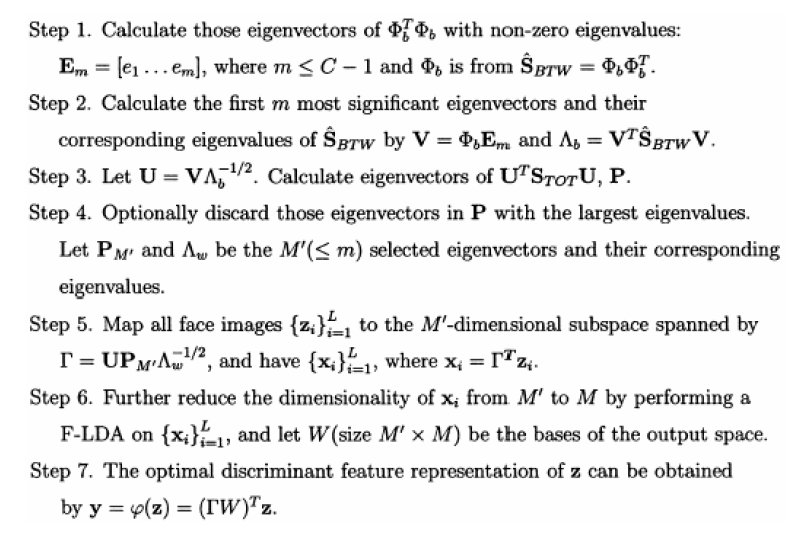
\includegraphics[width=\columnwidth]{img/step.png}
\caption{The algorithme - LDA}
\end{figure}

\subsection{Independent Component Analysis (ICA)}
	PCA is an optimal technique to search a reduced representation that minimizes error
reconstruction, the basis vectors taking into account the reconstruction error
may not be optimal for encoding information appropriate to the image
classification. The independent component analysis ICA is a generalization of PCA, the higher order statistics, which can
produce a more powerful data representation.
The goal of ICA is to find basis vectors localized in space and are statistically independent, minimizing the statistical dependence.


\subsection{Learning Vector Quantization (LVQ)}
The application of artificial neural networks in face recognition is for solve several problems face recognition and
classification of facial expressions.
A neural network is a system of information processing that was developed
as generalizations of mathematical models matching human knowledge. They
consist of interconnected processing units called neurons,
working together for perform a given task.
A neural network is a distributed parallel work. It resembles the human brain in three
aspects: knowledge is acquired by the network through a learning process, strengths
connection connected together, and each neuron has an internal state called threshold or function
activation used to classify the vectors.

A classification by neural network comprises the following steps:
\begin{itemize}
\item First a pre-learning image processing and association with each learning image (network input) an output vector, then comes the stage initialization (creation of network layers). 
\item It makes learning (supervised) in the network,
until it reaches a certain minimal error (the network learns to classify the images well
learning). 
\item We then present a new image to the network to identify (phase
recognition or activation or simulation of the network) that is ultimately assigned to a
given class . 
\end{itemize}

\subsection{Template matching}
The template matching technique is a global face recognition. The correlation
is generally used to measure the similarity between a template wich is a mask and stored
image to recognize. The templates should be deliberately designed to cover the variety
possible variations of the image.
While searching in the image, scale and rotation should also be
carefully considered to accelerate the process.
This technique was also used to locate the salient features "salient
features "such as eyes nose and mouth in a face image.

The template matching algorithm:
\begin{itemize}
\item Acquisition, reading and standardization of training images.
\item Calculates the average face of each class of persons (templates).
\item Acquired the reading and the normalization of the image audit.
\item Calculates the differences between the verification image and the template (the differences are images).
Is calculated based on amount of these differences (sum of pixel image difference).
\item And finally the minimum amount which will reference the class belongs image verification.
\end{itemize}

\subsection{characteristic points method}
\subsubsection{Cross ratio}[h]
	\begin{figure}
	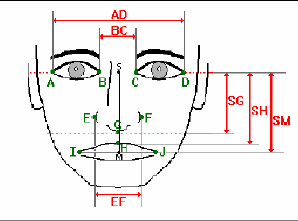
\includegraphics[width = \columnwidth]{img/ratio.png}
	\caption{Face ratios}
	\end{figure}
	The first local recognition methods were based on the width of the head, and
the distances between the eyes and mouth, by calculating the relationship between these distances. These methods are easily affected by irrelevant information.
The recognition algorithm using the Cross Ratio:
\begin{itemize}
\item Extraction of facial characteristic points (affected by the orientation of the head).
\item Definition of Cross Ratio for each 4 points of a line (distances
invariable). 
\item Make the correction of the location of characteristic points by
the application of symmetry and the cross ratio. 
\item Normalize after the feature vector:
N = F / | | F | |
\item And finally we use the Euclidean distance as a similarity measure.
\end{itemize}


\subsubsection{Elastic Graph Matching}
	\begin{figure}[h]
	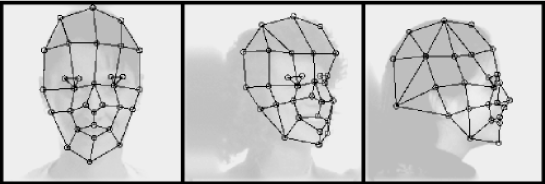
\includegraphics[width = \columnwidth]{img/egm.png}
	\caption{Elastic Graph Representation}
	\end{figure}
	The algorithm EGM "Elastic Graph Matching" represents individual faces a rectangular graph. Each node
	graph labeled with a set of complex coefficients of the Gabor wavelets
	called jets different orientations and scales. A jet is used to represent
	 face images based on wavelet transform
	Gabor. Only the magnitudes of coefficients are used for recognition.

	To recognize a new face, each graph of the database is adjusted to
	this new graph constructed, and the good fit indicates the recognized person.
	Initial results obtained encourage the use of faces with wide rotation
	angles. DLA is generally good in terms of variation of rotation, however,
	recognition process or adjustment is costly in computation.
	The EGM uses the phase of the complex coefficients of Gabor wavelets to achieve a
	more precise localization of the nodes and to differentiate between similar models in their
	coefficients of magnitude.
	The use of graphs EGM adaptive object "Adaptive object graphs," whose nodes
	referring to specific facial landmarks, or fiducial points "fiducial points" in
	face, namely the pupils, the corners of the mouth and nose.

\subsection{So ...}
We can see that the domain of researches in face recognition is very large. In each of these method, searchers work hard to find more an more best methods. A lot of team around the world are working about this subject.
	
		


